% MVP
\section{Minimum Viable Product}

\paragraph{} You can see a complete diagram of the user workflow in figure \ref{fig:workflow}, in this section we will display the features of the first mvp.

\subsection{Granular skills and the Wikipedia API}
\paragraph{} Arckane takes advantage of the implicit ontology or "network of concepts" which has Wikipedia, an ontology creates a common formalization of concepts, basically every article in Wikipedia becomes a potential skill or unit of knowledge to be used for the matchmaking between tutors and apprentices, so for example if someone wants to learn/teach how to swim he can declare it by searching in Arckane the keyword "Swimming (Sport)" (which is an article retrieved from Wikipedia) and make no ambiguation between someone who might want to learn/teach swimming as an aquatic locomotion physical phenomena. Also this lets us be as general or specific as desired, for example one may already know how to swim but wants to learn new swimming strokes, there is an article in Wikipedia called "Swimming Stroke" which adds the semantic to what he is specifically looking for, or even if he wants a tutor just to learn the butterfly stroke he can search it because there is a concrete article named "Butterfly Stroke". Arckane retrieves this information using the open Wikimedia API which allows our servers to query Wikipedia. Also Arckane will eventually work in its own powerful Ontology adding a lot of semantics to what is being learned and teached, this way we can add Artificial Intelligence features later on.

\subsection{The apprentice profile}
\paragraph{} The mvp must have a profile for each user, in the profile anyone can publicly see what he has learned as an apprentice and what he is teaching as a tutor. In this version in the case of the apprentice section we will see a list of the skills a tutor has rated him on (and the rating) and which skills he have declared he wishes to learn.

\subsection{The tutor profile}
\paragraph{} In the tutor section we will see:
\begin{itemize}
  \item A self written description of who he is and how he likes to teach.
  \item A label telling if the tutor is teaching remotely, locally (physical presence) or both.
  \item A map showing in which area he is teaching (if he is teaching locally).
  \item The hourly rate.
  \item A label telling up to how many apprentices he wishes to take at a given moment.
\end{itemize}

\subsection{Setting up as a tutor}
\paragraph{} Every user will be able to set up his account to become a tutor, all he should need to do is three steps, add his information as a tutor (description, skills he is willing to teach, etc.), add his information for payments and his hourly rate, and finally tell Arckane his available schedule to appoint sessions.

\subsection{Searching and choosing a tutor}
\paragraph{} A search box should be available to start writting a keyword, Arckane will return a list of concepts or Wikipedia article titles which may match the keyword, the user can tap this results to skim through a list of tutors that can teach those skills. A button should filter between local tutors, remote tutors or both. Now here there are two possibilities, there can be no tutors nearby or remotely which teach that skill or there can be:

\paragraph{There were no available tutors case} then the user is shown a message saying there were no matching tutors, then the user is asked if he wishes to be notified via email if  new tutors are matched in the future.

\paragraph{There were available tutors case} then the user is displayed with a list of cards showing the resume information and hourly rates of the matched tutors, these cards can be opened to show the full profile of the tutors, then the user can tap to schedule a teacher, Arckane does NOT show the teacher's schedule, but proposes the user good times to schedule the session. For scheduling the process is as follows: 1) the tutor tells Arckane his free times, 2) an apprentice chooses a tutor and set ups directly with Arckane (Arckane does not reveal the tutors schedule), 3) the tutor is notified about the new session, which he has to confirm.

\subsection{Payments}
\paragraph{} The payment process goes as follows: 1) When choosing the tutor the apprentice pays the hourly rate to Arckane, 2) the session is executed, 3) if the apprentice is satisfied with the session Arckane pays the tutor and charges the tutor and apprentice fees, 4) if not Arckane returns the money to the apprentice and does not charge any fee.

\subsection{Apprentice and tutor ratings}
\paragraph{} After the scheduling is successful the session should be executed, Arckane will ask if the session was successful after it has theoretically been finished, to the apprentice it asks if he was happy with the session and to rate the tutor. To the tutor it will prompt him to rate the skills of the apprentice, after the rating Arckane will sum the time of the session to the skills of the apprentice.

\subsection{Chosen technologies}
\paragraph{} (More detailed information can be found in the section \ref{system_architecture} System Architecture) In this version we are exploiting the power of Polymer, Google’s framework to use HTML5’s web components technology, this allows us to create a modern, responsive web application which adapts its interface to mobile or desktop easily and with almost no technical hassle. With this we can create a powerful web application that serves every platform. In section  \ref{system_architecture} can be found in detail the back-end and front-end technologies being used (including the database and deployment environment) and also the general architecture of the system.

% Workflow figure
\pagebreak % New page
\newgeometry{top=0.1in,bottom=1in,right=0.1in,left=0.1in} % Change page margins
\begin{figure}[h] % Figure
    \centering
    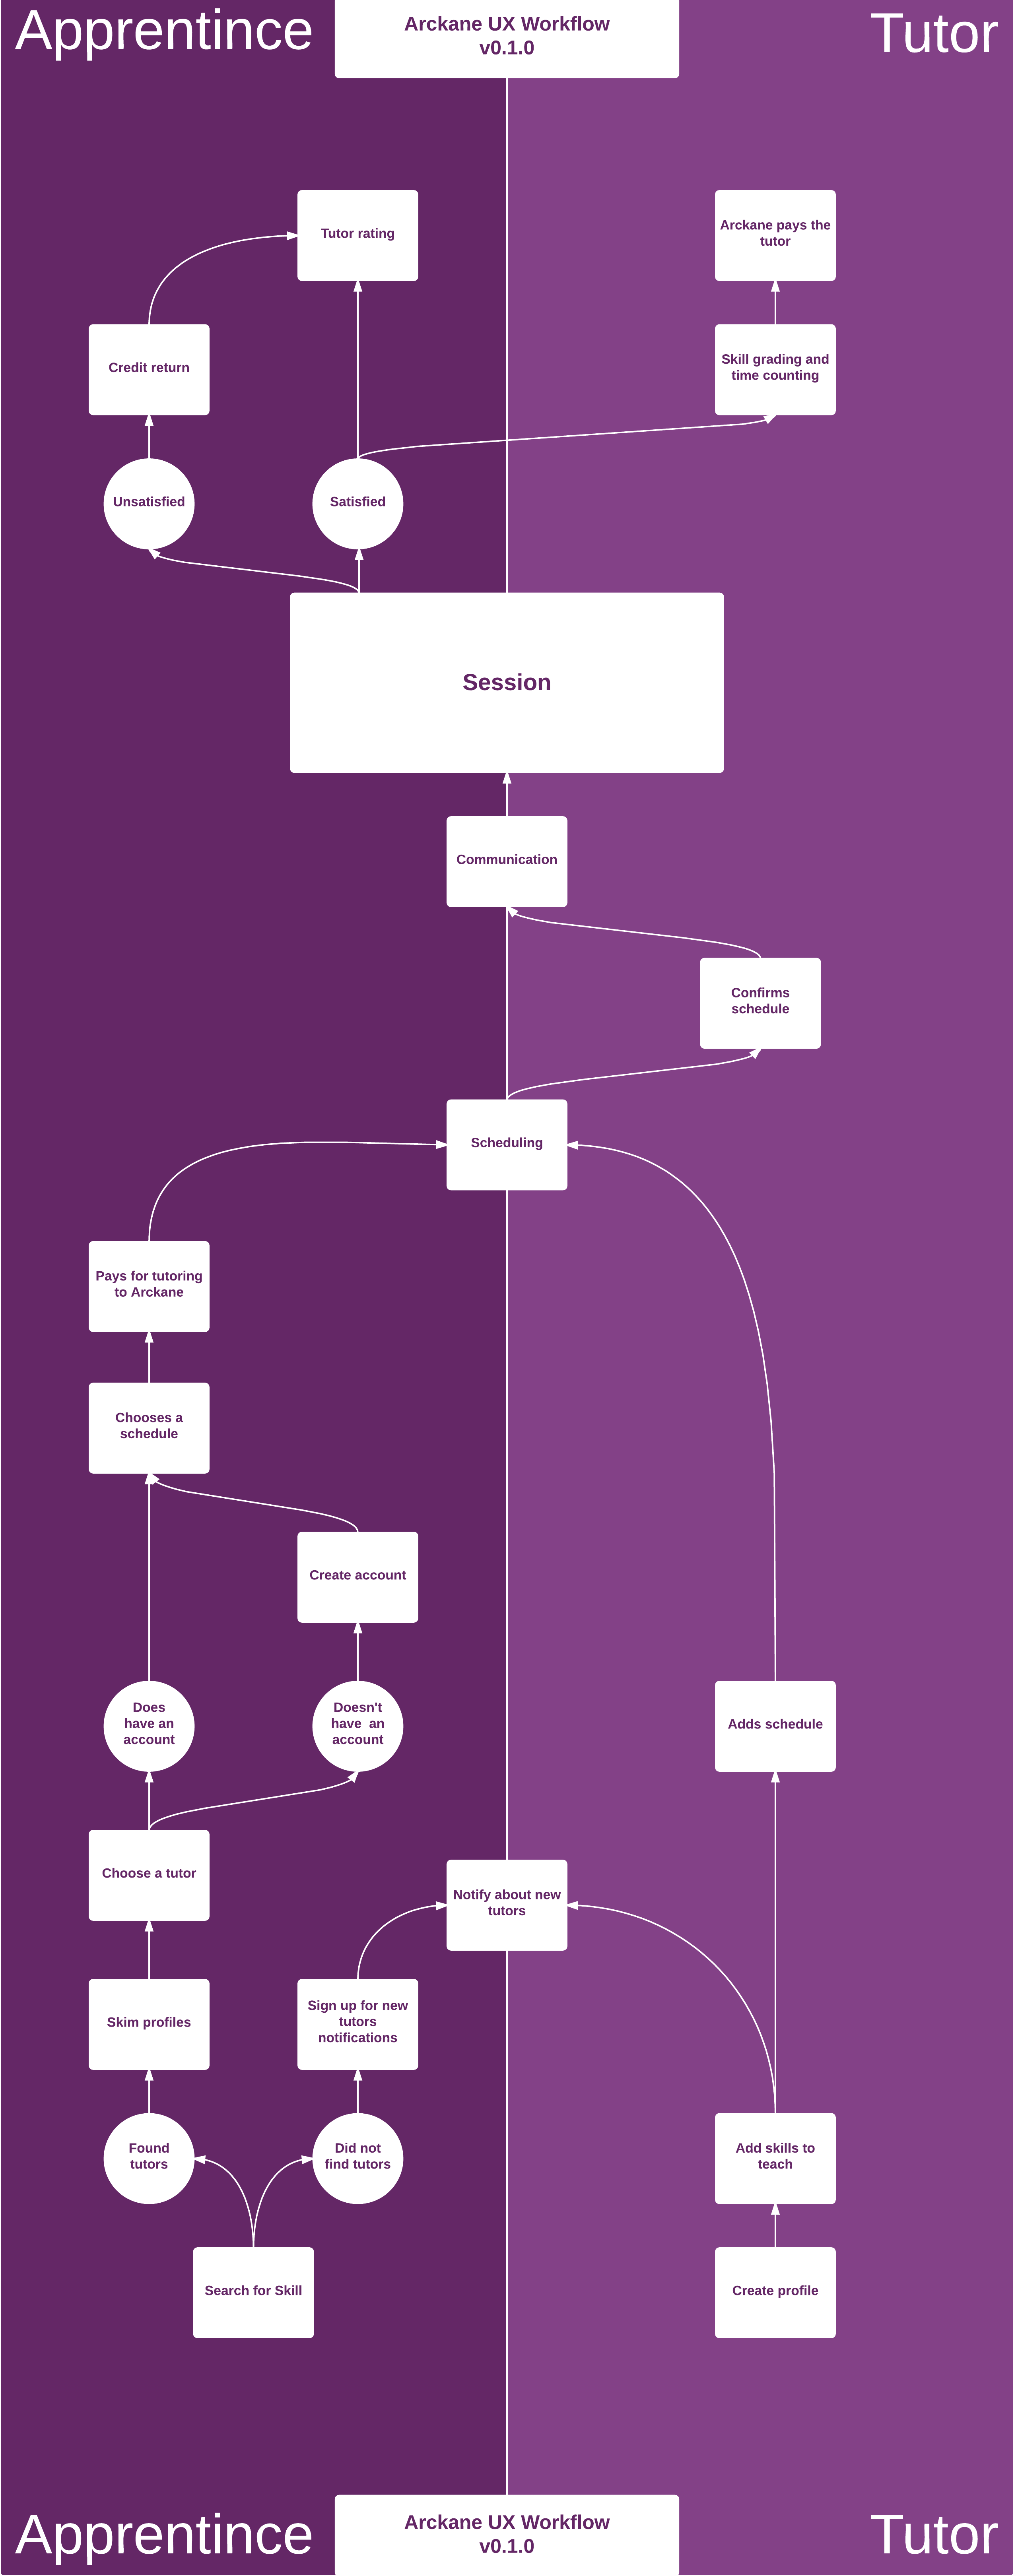
\includegraphics[height=\textheight]{workflow}
    \caption{Arckane UX Workflow v0.1}
    \label{fig:workflow}
\end{figure}
\restoregeometry % Restore page margins
\pagebreak


